\documentclass{IOS-Book-Article}
\usepackage{mathptmx}
\usepackage{multirow}
\usepackage{graphicx}
\usepackage[utf8]{inputenc}
\usepackage[T1]{fontenc}
\usepackage[english]{babel}
\begin{document}
\begin{frontmatter}
\title{Measuring the competence of LLMs in Brazilian law}
\author[A]{\fnms{Eduardo} \snm{Pacheco}}
and
\author[A]{\fnms{Cibele Maria} \snm{Russo}}
\runningauthor{E. Pacheco and C. M. Russo}
\address[A]{Instituto de Ciências Matemáticas e de Computação, Universidade de São Paulo}
\begin{abstract}
Evaluating open-ended legal answers at scale depends on using a language model as the grader, and choosing which model will grade is done by measuring its agreement with human annotation and ordering the candidates in a table. We measure 31 models in the three roles this arrangement involves, over the same 105 questions from the second stage of the OAB Bar Exam and the same 940 criteria of the official grading guidelines, with a gold standard from 3 legal experts: as respondents on the discursive question, as respondents on drafting a legal document, and as judges of the other models' answers. The three orderings are reported by area of law. There are 3 results. Judging and answering are associated competences, but the association weakens as the task stops demanding form and starts demanding substance: $\rho$ = 0.67 on the discursive question, 0.61 on the formal criteria of the document and 0.41 on the substantive ones. Drafting a document is not a single task: split into the two classes of criterion the examining board itself labels, the judge's agreement is higher on the formal part than on the substantive one for \textbf{25 of the 26} judges measured, with a median difference of 0.168, the two orderings agree only at $\rho$ = 0.48, and the leader is not the same. And a single number per judge hides more than it shows: among the top nine, whom the protocol's noise floor ties within a span of 0.047, a single judge's agreement varies across areas of law with a median of \textbf{0.279}, almost 6 times that span.
\end{abstract}
\begin{keyword}
Benchmark \sep LLM-as-a-Judge \sep Brazil \sep Law \sep Reproducibility
\end{keyword}
\end{frontmatter}

\section{Introduction}

Evaluating whether a language model answered an open legal question well is expensive. There is no single answer key, and string comparison does not work, because two correct answers may not share a word. The human alternative, hiring lawyers to read every answer, does not scale to dozens of models over hundreds of questions. The route the field has taken is to use a language model as the grader, the technique known as \emph{LLM-as-judge} [1]. The grader is given the question, the answer under evaluation and the grading criterion, and is asked for a verdict. This makes scale possible, but pushes the problem one step back: how do we know the grader grades well? The standard answer is to calibrate it against human annotation. Lawyers annotate a sample, the agreement between each candidate model and that annotation is measured, and the one that agrees most is chosen. Agreement is measured by Cohen's $\kappa$ [7], the proportion of matches discounted by the agreement expected by chance. The discount matters: if 80\% of criteria have the answer "not met", a judge that always answers "not met" matches 80\% while knowing nothing, and its $\kappa$ is zero. By the field's convention, $\kappa$ above 0.80 counts as strong agreement. This arrangement puts models in three distinct roles over the same material: drafting a legal document, answering a discursive question, and judging what the others wrote. Current practice treats the three as a single competence, and that is what licenses choosing the judge by its performance on the task, without human annotation.

This work measures the same 31 models in the three roles, over the same set of questions and the same grading guidelines, and reports each role by area of law. The three results that follow are consequences of that joint measurement, and none of them appears in an aggregate table of one number per model. The verdicts of the 31 candidates over the 940 criteria, in up to 5 repetitions each, and the annotations of the three legal experts that form the gold standard are deposited at \texttt{10.5281/zenodo.22739161} [11], with a checksum per file. The training corpus and the judgments of the 180 conditions of the companion study [10] are at \texttt{10.5281/zenodo.22739216} [12] and \texttt{10.5281/zenodo.22739184} [13], and the code at [14].

\section{Related work}

The use of models as evaluators was systematised by Zheng et al. [1], who also documented biases of the procedure, of position, of verbosity and of self-preference. Later work measured the judge's agreement with humans in specific domains and proposed corrections, but the reporting format stayed the same: an agreement table, ordered, with one number per judge. In legal evaluation, LegalBench [2] avoids the problem by using short, verifiable answer tasks, at the cost of moving away from professional practice.

For legal Portuguese there are 3 directly relevant evaluation sets, all built on real examinations, and two of them on the same one we use. \textbf{oab-bench} [3] draws 105 questions across seven areas of law from recent editions of the OAB Bar Exam and grades them on a 0--10 scale against the examiners' guidelines, reporting a strong correlation between a frontier model's scores and human ones. \textbf{Magis-Bench} [4] moves to the judiciary, with 74 questions from eight competitive examinations for judicial positions between 2023 and 2025, covering discursive analysis and the drafting of civil and criminal judgments, graded by four frontier models acting as judges. \textbf{Rabula} [5] is built on the 2024 OAB Bar Exam with four tasks, grades the generative ones against the board's own criteria as binary questions weighted by difficulty, and calibrates the automatic judge by Cohen's agreement with 3 legal experts. From the last of these we inherit the evaluation set, the human gold standard and the grading procedure, without modifying them.

All three report model competence as an aggregate score per task, and Rabula also reports the judge's agreement as one number per candidate. None of them splits document drafting into the classes of criterion the board labels, nor reports agreement by area of law, nor measures the same models as respondents and as judges to compare the two orderings. On the reproducibility of inference, it is known that the non-associativity of floating-point arithmetic makes the result depend on how operations are grouped [6]; what we did not find in the \emph{LLM-as-judge} literature is the recognition that this makes batch size a parameter of the protocol, alongside temperature and seed.

\section{Materials and methods}

\subsection{The two tasks and what each one demands}

The evaluation set consists of \textbf{105 questions} from the second stage of the OAB Bar Exam, drawn from editions 39, 40 and 41, 35 from each. They cover seven areas of law with exactly 15 questions each, so that no area dominates the mean. There are 84 discursive questions and 21 practical cases that ask for a legal document to be drafted, and the two genres demand different things.

The \textbf{discursive question} presents a short case, a median of 182 words, and asks two to four objective questions of law about it. An administrative law case from edition 41 describes the expropriation of rural property by the federal government and asks whether the public authority must make an offer of compensation before filing suit and whether arbitration is available in the procedure. The expected answer is short and the guidelines break it into few criteria, a median of 4 and at most 7: one requires the correct thesis, "the public authority must notify the owner and present an offer of compensation before filing", worth 0.5 points, and another requires the legal basis, "under Art. 10-A of Decree-Law 3,365/1941", worth 0.1. What is demanded is legal content, with no documentary form to satisfy.

\textbf{Drafting a legal document} presents a longer case, a median of 399 words, and asks for a complete procedural document written as counsel for one of the parties. The guidelines break the document into many more criteria, a median of 26 and up to 38, and these come labelled with a title. In a writ of mandamus against an act of the chair of a procurement committee, the first criteria are "Addressing: the document must be addressed to the Civil Court or the Public Treasury Court of the district", "Identification of the parties: respondent authority, João da Silva, chair of the Procurement Committee" and "Admissibility: there was a violation of a clear and certain right". Beyond legal content, the skeleton of the document is demanded.

\begin{table}[!ht]
\centering
\caption{Composition of the evaluation set and of the human gold standard. The unit of analysis is not the question but the \textbf{criterion}, a binary assertion about the answer extracted from the official grading guidelines.}
\footnotesize\setlength{\tabcolsep}{2pt}
\begin{tabular}{llrrrr}
\hline
\textbf{Genre} & \textbf{Questions} & \textbf{Criteria} & \textbf{formal} & \textbf{substantive} & \textbf{$\kappa$ among humans} \\
\hline
Discursive question & 84 & 379 & -- & 379 & 0.789 \\
Document drafting & 21 & 561 & 148 & 413 & 0.763 \\
\hline
\end{tabular}
\end{table}


\subsection{The two classes of criterion in document drafting}

The titles with which the board labels the document criteria fall into two families. Those of \textbf{form} cover the skeleton of the document: addressing to the competent court, identification of the parties, timeliness, admissibility requirements, closing with place, date and signature. Those of \textbf{substance} cover the legal thesis, the grounds and the requests. There are 148 and 413 of them respectively, and every formal criterion is in a document, because discursive questions have no documentary skeleton to satisfy. Grouping the titles into the two families is ours; the titles are not. The split matters because the two classes demand different cognitive operations, both from whoever writes and from whoever grades. Deciding whether the document was addressed to the competent court is matching a stretch of text against a short key. Deciding whether there was a violation of a clear and certain right is assessing a thesis. There is no reason to assume a single model is equally good at both, and Section 4.3 shows it is not.

\subsection{The three roles and the measurement protocol}

Each of the 31 models was measured in the three roles. As a \textbf{respondent}, it receives the case and produces the answer or the document, which is graded against the guidelines by the calibrated pipeline, and the score is the percentage of the board's points, weighted by the points of each criterion. As a \textbf{judge}, it receives another model's answer and one criterion, and returns a binary verdict, compared against the gold standard of \textbf{940 decisions} taken by 3 experienced lawyers, inherited from Rabula [5]. Agreement is measured by Cohen's $\kappa$, separately by genre, by class of criterion and by area of law.

The whole protocol was repeated \textbf{up to 5 times} per candidate, with the code frozen, with no change of prompt, of library or of model version between repetitions. It is this repetition that allows the dispersion of $\kappa$ under an identical protocol to be measured, and from it the decision threshold used below is derived. Coverage is not uniform across candidates: 26 judges completed the 5 repetitions, three completed three because of API quota, and two produced no usable result on document drafting. A judge is scored only if it covers at least 85\% of the criteria of the genre, and only if what is missing is missing by chance, which is checked by Fisher's exact test on the table of judged against omitted by positive against negative human answer.

\section{Results}

Tables 2 and 3 give each judge's agreement with the human gold standard, by area of law, one per genre, with document drafting split into the two classes of criterion. Tables 4 and 5 give, in the same layout, the score of the same models as respondents. The tables show the 22 judges with the best agreement on document substance, which is what fits on the page; the 26 that produced a result in all three tasks are in the deposit [11], with the same decomposition. \textbf{Every statistic reported below is computed over the 26}, not over the displayed subset, which is selected on one of the variables at issue.

\begin{table}[!ht]
\centering
\caption{Cohen's agreement with the human gold standard on the \textbf{discursive question}, by area of law. Values $\times$100. The \textbf{range} column is the distance between the best and the worst area of the same judge.}
\footnotesize\setlength{\tabcolsep}{2pt}
\begin{tabular}{llrrrrrrrr}
\hline
\textbf{Judge} & \textbf{Admin.} & \textbf{Civil} & \textbf{Const.} & \textbf{Corp.} & \textbf{Crim.} & \textbf{Labour} & \textbf{Tax} & \textbf{overall} & \textbf{range} \\
\hline
\texttt{claude-opus-4-6} & 78 & 74 & 92 & 74 & 88 & 73 & 82 & 80 & 18 \\
\texttt{gpt-oss-120b} & 72 & 78 & 89 & 78 & 85 & 76 & 93 & 82 & 21 \\
\texttt{claude-opus-4-5} & 82 & 81 & 91 & 78 & 84 & 77 & 82 & 82 & 13 \\
\texttt{kimi-k2-5} & 83 & 83 & 81 & 78 & 70 & 74 & 88 & 80 & 18 \\
\texttt{kimi-k2-thinking} & 80 & 81 & 85 & 77 & 81 & 76 & 85 & 81 & 9 \\
\texttt{glm-4-7} & 71 & 85 & 86 & 85 & 77 & 81 & 86 & 82 & 15 \\
\texttt{claude-sonnet-4-5} & 63 & 88 & 86 & 73 & 87 & 81 & 75 & 81 & 25 \\
\texttt{sabia-4} & 72 & 84 & 92 & 79 & 81 & 77 & 88 & 82 & 19 \\
\texttt{claude-sonnet-4-6} & 64 & 77 & 96 & 73 & 79 & 77 & 69 & 77 & 32 \\
\texttt{claude-haiku-4-5} & 65 & 79 & 74 & 81 & 82 & 75 & 80 & 77 & 17 \\
\texttt{deepseek-v3} & 63 & 81 & 82 & 77 & 79 & 82 & 74 & 78 & 20 \\
\texttt{glm-5} & 66 & 85 & 87 & 78 & 71 & 87 & 80 & 80 & 21 \\
\texttt{minimax-m2-5} & 78 & 74 & 85 & 83 & 77 & 85 & 89 & 81 & 15 \\
\texttt{qwen3-235b-vl} & 71 & 84 & 78 & 88 & 69 & 74 & 79 & 78 & 19 \\
\texttt{mistral-l3-675b} & 62 & 82 & 79 & 83 & 70 & 81 & 83 & 77 & 21 \\
\texttt{mistral-large} & 82 & 80 & 83 & 84 & 70 & 67 & 83 & 79 & 17 \\
\texttt{magistral-small} & 68 & 80 & 67 & 79 & 45 & 69 & 86 & 70 & 41 \\
\texttt{nemotron-s3-120b} & 70 & 69 & 59 & 88 & 46 & 46 & 67 & 63 & 43 \\
\texttt{sabiazinho-4} & 70 & 77 & 88 & 82 & 67 & 71 & 82 & 76 & 22 \\
\texttt{qwen3-80b-a3b} & 64 & 82 & 80 & 78 & 42 & 69 & 86 & 71 & 44 \\
\texttt{llama4-maverick} & 84 & 79 & 86 & 84 & 59 & 77 & 84 & 79 & 27 \\
\texttt{qwen3-32b} & 74 & 76 & 62 & 80 & 61 & 67 & 78 & 71 & 20 \\
\hline
\end{tabular}
\end{table}


\begin{table}[!ht]
\centering
\caption{Cohen's agreement with the human gold standard on \textbf{drafting a legal document}, by area of law. Each cell carries two values, \textbf{formal} | substantive, for the two classes of criterion the examining board labels. Values $\times$100. The \textbf{range} column is the distance between the best and the worst area of the same judge.}
\footnotesize\setlength{\tabcolsep}{2pt}
\begin{tabular}{llrrrrrrrr}
\hline
\textbf{Judge} & \textbf{Admin.} & \textbf{Civil} & \textbf{Const.} & \textbf{Corp.} & \textbf{Crim.} & \textbf{Labour} & \textbf{Tax} & \textbf{overall} & \textbf{range} \\
\hline
\texttt{claude-opus-4-6} & \textbf{89}|76 & \textbf{64}|69 & \textbf{91}|76 & \textbf{75}|57 & \textbf{65}|80 & \textbf{78}|73 & \textbf{91}|87 & \textbf{80}|74 & \textbf{27}|30 \\
\texttt{gpt-oss-120b} & \textbf{84}|73 & \textbf{78}|74 & \textbf{72}|57 & \textbf{75}|67 & \textbf{65}|73 & \textbf{77}|76 & \textbf{88}|85 & \textbf{78}|73 & \textbf{23}|28 \\
\texttt{claude-opus-4-5} & \textbf{91}|66 & \textbf{78}|65 & \textbf{91}|76 & \textbf{87}|62 & \textbf{75}|84 & \textbf{80}|67 & \textbf{88}|87 & \textbf{85}|73 & \textbf{16}|25 \\
\texttt{kimi-k2-5} & \textbf{80}|59 & \textbf{78}|77 & \textbf{74}|60 & \textbf{64}|66 & \textbf{69}|81 & \textbf{79}|61 & \textbf{88}|90 & \textbf{77}|72 & \textbf{24}|31 \\
\texttt{kimi-k2-thinking} & \textbf{82}|63 & \textbf{57}|74 & \textbf{72}|59 & \textbf{68}|65 & \textbf{67}|73 & \textbf{86}|61 & \textbf{93}|93 & \textbf{77}|71 & \textbf{36}|34 \\
\texttt{glm-4-7} & \textbf{87}|63 & \textbf{78}|69 & \textbf{82}|53 & \textbf{73}|63 & \textbf{75}|84 & \textbf{78}|71 & \textbf{88}|86 & \textbf{81}|70 & \textbf{15}|33 \\
\texttt{claude-sonnet-4-5} & \textbf{98}|61 & \textbf{78}|72 & \textbf{91}|62 & \textbf{87}|60 & \textbf{65}|79 & \textbf{79}|60 & \textbf{88}|86 & \textbf{84}|70 & \textbf{33}|26 \\
\texttt{sabia-4} & \textbf{82}|68 & \textbf{66}|67 & \textbf{84}|59 & \textbf{87}|62 & \textbf{85}|80 & \textbf{79}|60 & \textbf{88}|85 & \textbf{82}|70 & \textbf{22}|26 \\
\texttt{claude-sonnet-4-6} & \textbf{85}|57 & \textbf{78}|72 & \textbf{91}|71 & \textbf{75}|60 & \textbf{75}|83 & \textbf{80}|56 & \textbf{88}|79 & \textbf{83}|70 & \textbf{16}|27 \\
\texttt{claude-haiku-4-5} & \textbf{85}|52 & \textbf{76}|70 & \textbf{74}|53 & \textbf{68}|69 & \textbf{87}|73 & \textbf{78}|57 & \textbf{88}|85 & \textbf{80}|66 & \textbf{20}|33 \\
\texttt{deepseek-v3} & \textbf{91}|55 & \textbf{78}|63 & \textbf{77}|49 & \textbf{87}|63 & \textbf{75}|78 & \textbf{81}|58 & \textbf{88}|85 & \textbf{83}|65 & \textbf{16}|36 \\
\texttt{glm-5} & \textbf{91}|59 & \textbf{78}|53 & \textbf{82}|51 & \textbf{82}|68 & \textbf{73}|79 & \textbf{83}|62 & \textbf{88}|84 & \textbf{83}|65 & \textbf{18}|32 \\
\texttt{minimax-m2-5} & \textbf{75}|57 & \textbf{63}|64 & \textbf{79}|43 & \textbf{73}|58 & \textbf{73}|79 & \textbf{92}|59 & \textbf{88}|79 & \textbf{79}|63 & \textbf{29}|35 \\
\texttt{qwen3-235b-vl} & \textbf{91}|48 & \textbf{73}|59 & \textbf{72}|42 & \textbf{87}|62 & \textbf{75}|70 & \textbf{80}|65 & \textbf{88}|78 & \textbf{81}|61 & \textbf{19}|36 \\
\texttt{mistral-l3-675b} & \textbf{89}|54 & \textbf{71}|53 & \textbf{83}|42 & \textbf{79}|55 & \textbf{87}|75 & \textbf{86}|64 & \textbf{88}|81 & \textbf{84}|61 & \textbf{18}|39 \\
\texttt{mistral-large} & \textbf{81}|44 & \textbf{66}|66 & \textbf{63}|43 & \textbf{59}|59 & \textbf{75}|64 & \textbf{86}|66 & \textbf{88}|76 & \textbf{76}|61 & \textbf{29}|33 \\
\texttt{magistral-small} & \textbf{76}|45 & \textbf{82}|50 & \textbf{72}|35 & \textbf{62}|59 & \textbf{79}|72 & \textbf{87}|64 & \textbf{88}|64 & \textbf{80}|56 & \textbf{26}|37 \\
\texttt{nemotron-s3-120b} & \textbf{65}|46 & \textbf{76}|54 & \textbf{77}|31 & \textbf{61}|61 & \textbf{71}|60 & \textbf{87}|58 & \textbf{75}|72 & \textbf{75}|55 & \textbf{25}|41 \\
\texttt{sabiazinho-4} & \textbf{35}|59 & \textbf{37}|40 & \textbf{37}|54 & \textbf{36}|32 & \textbf{63}|74 & \textbf{63}|39 & \textbf{57}|71 & \textbf{51}|54 & \textbf{28}|42 \\
\texttt{qwen3-80b-a3b} & \textbf{64}|36 & \textbf{58}|48 & \textbf{62}|35 & \textbf{57}|59 & \textbf{65}|53 & \textbf{79}|57 & \textbf{88}|68 & \textbf{69}|51 & \textbf{31}|34 \\
\texttt{llama4-maverick} & \textbf{64}|54 & \textbf{88}|43 & \textbf{68}|28 & \textbf{87}|54 & \textbf{78}|49 & \textbf{89}|56 & \textbf{88}|66 & \textbf{81}|50 & \textbf{26}|38 \\
\texttt{qwen3-32b} & \textbf{73}|46 & \textbf{61}|35 & \textbf{56}|38 & \textbf{83}|51 & \textbf{84}|56 & \textbf{86}|59 & \textbf{88}|58 & \textbf{77}|49 & \textbf{32}|24 \\
\hline
\end{tabular}
\end{table}


\begin{table}[!ht]
\centering
\caption{Score of the same models as \textbf{respondents} on the discursive question, by area of law.}
\footnotesize\setlength{\tabcolsep}{2pt}
\begin{tabular}{llrrrrrrr}
\hline
\textbf{Model} & \textbf{Admin.} & \textbf{Civil} & \textbf{Const.} & \textbf{Corp.} & \textbf{Crim.} & \textbf{Labour} & \textbf{Tax} & \textbf{overall} \\
\hline
\texttt{claude-opus-4-6} & 94.9 & 91.2 & 89.6 & 85.2 & 87.5 & 93.5 & 79.2 & 88.8 \\
\texttt{gpt-oss-120b} & 55.1 & 60.9 & 40.9 & 42.9 & 53.7 & 50.6 & 41.3 & 49.3 \\
\texttt{claude-opus-4-5} & 93.8 & 87.4 & 87.3 & 87.8 & 85.7 & 95.2 & 83.2 & 88.6 \\
\texttt{kimi-k2-5} & 64.3 & 61.9 & 58.7 & 43.1 & 63.6 & 61.7 & 47.4 & 57.2 \\
\texttt{kimi-k2-thinking} & 53.9 & 47.7 & 54.6 & 52.6 & 48.4 & 50.9 & 42.4 & 50.6 \\
\texttt{glm-4-7} & 60.0 & 67.7 & 69.4 & 47.7 & 70.2 & 66.7 & 56.5 & 62.6 \\
\texttt{claude-sonnet-4-5} & 77.9 & 85.9 & 80.7 & 54.8 & 77.1 & 80.7 & 64.9 & 74.6 \\
\texttt{sabia-4} & 72.3 & 80.7 & 70.2 & 64.9 & 85.8 & 91.1 & 74.0 & 77.0 \\
\texttt{claude-sonnet-4-6} & 90.0 & 82.3 & 84.9 & 73.9 & 81.7 & 85.8 & 84.4 & 83.3 \\
\texttt{claude-haiku-4-5} & 60.0 & 65.4 & 54.1 & 50.8 & 57.1 & 48.9 & 46.6 & 54.7 \\
\texttt{deepseek-v3} & 73.1 & 64.3 & 68.0 & 55.1 & 69.2 & 49.6 & 45.7 & 60.7 \\
\texttt{glm-5} & 63.5 & 69.8 & 64.7 & 42.6 & 71.1 & 62.4 & 61.7 & 62.3 \\
\texttt{minimax-m2-5} & 62.3 & 73.2 & 71.7 & 49.4 & 70.4 & 57.8 & 57.8 & 63.0 \\
\texttt{qwen3-235b-vl} & 60.4 & 64.4 & 58.7 & 53.7 & 61.4 & 56.8 & 36.2 & 56.0 \\
\texttt{mistral-l3-675b} & 68.8 & 79.0 & 66.8 & 66.6 & 77.3 & 78.7 & 61.4 & 71.2 \\
\texttt{mistral-large} & 38.6 & 28.9 & 18.4 & 47.3 & 43.4 & 32.4 & 26.5 & 33.7 \\
\texttt{magistral-small} & 48.1 & 51.8 & 46.9 & 44.5 & 60.2 & 47.7 & 39.8 & 48.4 \\
\texttt{nemotron-s3-120b} & 53.8 & 53.5 & 46.7 & 47.6 & 53.9 & 49.3 & 46.6 & 50.2 \\
\texttt{sabiazinho-4} & 56.3 & 78.7 & 71.7 & 61.1 & 76.1 & 81.1 & 62.0 & 69.6 \\
\texttt{qwen3-80b-a3b} & 55.5 & 54.8 & 53.9 & 48.2 & 57.8 & 48.5 & 52.1 & 53.0 \\
\texttt{llama4-maverick} & 54.9 & 62.6 & 69.2 & 44.1 & 65.2 & 59.4 & 54.3 & 58.5 \\
\texttt{qwen3-32b} & 38.1 & 38.9 & 28.8 & 34.7 & 44.4 & 29.2 & 31.2 & 35.1 \\
\hline
\end{tabular}
\end{table}


\begin{table}[!ht]
\centering
\caption{Score of the same models as \textbf{respondents} on drafting a legal document, as a percentage of the board's points. Cells read as before: \textbf{formal} | substantive.}
\footnotesize\setlength{\tabcolsep}{2pt}
\begin{tabular}{llrrrrrrr}
\hline
\textbf{Model} & \textbf{Admin.} & \textbf{Civil} & \textbf{Const.} & \textbf{Corp.} & \textbf{Crim.} & \textbf{Labour} & \textbf{Tax} & \textbf{overall} \\
\hline
\texttt{claude-opus-4-6} & \textbf{68.5}|32.7 & \textbf{40.1}|66.7 & \textbf{68.8}|66.4 & \textbf{43.8}|59.6 & \textbf{50.0}|63.8 & \textbf{53.6}|55.5 & \textbf{70.8}|68.4 & \textbf{55.5}|63.4 \\
\texttt{gpt-oss-120b} & \textbf{53.1}|29.6 & \textbf{59.0}|55.8 & \textbf{48.4}|50.6 & \textbf{50.7}|50.5 & \textbf{18.5}|25.7 & \textbf{20.1}|54.7 & \textbf{48.0}|62.8 & \textbf{42.5}|47.1 \\
\texttt{claude-opus-4-5} & \textbf{68.5}|46.4 & \textbf{62.0}|65.0 & \textbf{63.1}|60.4 & \textbf{61.3}|48.1 & \textbf{51.9}|55.4 & \textbf{46.0}|70.3 & \textbf{57.8}|65.5 & \textbf{58.6}|58.7 \\
\texttt{kimi-k2-5} & \textbf{38.3}|19.7 & \textbf{40.6}|45.0 & \textbf{39.8}|38.9 & \textbf{47.4}|30.5 & \textbf{13.0}|27.0 & \textbf{13.8}|43.7 & \textbf{26.1}|44.3 & \textbf{31.3}|35.6 \\
\texttt{kimi-k2-thinking} & \textbf{29.0}|11.1 & \textbf{52.2}|15.4 & \textbf{45.9}|17.9 & \textbf{40.7}|8.2 & \textbf{0.0}|23.7 & \textbf{19.1}|13.9 & \textbf{27.4}|30.7 & \textbf{30.6}|15.8 \\
\texttt{glm-4-7} & \textbf{63.6}|57.1 & \textbf{82.1}|71.6 & \textbf{79.8}|75.2 & \textbf{69.1}|54.8 & \textbf{51.9}|59.0 & \textbf{53.1}|70.4 & \textbf{68.4}|70.1 & \textbf{66.9}|65.5 \\
\texttt{claude-sonnet-4-5} & \textbf{72.8}|26.9 & \textbf{61.2}|49.5 & \textbf{61.7}|50.7 & \textbf{52.4}|48.6 & \textbf{46.3}|41.9 & \textbf{39.9}|30.7 & \textbf{39.6}|62.0 & \textbf{53.4}|44.3 \\
\texttt{sabia-4} & \textbf{74.7}|26.6 & \textbf{54.7}|67.6 & \textbf{59.7}|54.6 & \textbf{61.3}|46.6 & \textbf{79.6}|53.6 & \textbf{43.2}|47.5 & \textbf{60.0}|53.3 & \textbf{61.9}|50.0 \\
\texttt{claude-sonnet-4-6} & \textbf{64.8}|39.6 & \textbf{52.8}|55.1 & \textbf{63.1}|58.8 & \textbf{65.0}|43.6 & \textbf{31.5}|51.9 & \textbf{30.3}|44.1 & \textbf{52.0}|58.7 & \textbf{51.4}|50.2 \\
\texttt{claude-haiku-4-5} & \textbf{35.2}|14.1 & \textbf{46.6}|53.1 & \textbf{47.5}|49.3 & \textbf{45.2}|29.2 & \textbf{3.7}|34.9 & \textbf{18.3}|30.7 & \textbf{46.2}|48.6 & \textbf{34.7}|37.1 \\
\texttt{deepseek-v3} & \textbf{38.9}|34.9 & \textbf{72.9}|62.8 & \textbf{57.4}|75.4 & \textbf{56.7}|59.1 & \textbf{33.3}|57.6 & \textbf{29.1}|55.4 & \textbf{57.3}|59.1 & \textbf{49.4}|57.8 \\
\texttt{glm-5} & \textbf{61.7}|48.5 & \textbf{82.5}|67.2 & \textbf{70.3}|67.8 & \textbf{73.7}|53.5 & \textbf{33.3}|71.0 & \textbf{37.4}|69.9 & \textbf{63.6}|62.0 & \textbf{60.4}|62.8 \\
\texttt{minimax-m2-5} & \textbf{54.3}|24.2 & \textbf{57.6}|48.4 & \textbf{57.4}|48.7 & \textbf{49.2}|41.1 & \textbf{38.9}|41.7 & \textbf{26.8}|44.8 & \textbf{44.6}|45.4 & \textbf{46.9}|42.0 \\
\texttt{qwen3-235b-vl} & \textbf{35.8}|34.7 & \textbf{76.9}|59.3 & \textbf{45.8}|64.2 & \textbf{65.4}|50.9 & \textbf{25.9}|45.1 & \textbf{33.9}|52.8 & \textbf{52.2}|54.7 & \textbf{48.0}|51.7 \\
\texttt{mistral-l3-675b} & \textbf{63.0}|58.1 & \textbf{78.4}|73.2 & \textbf{82.6}|77.7 & \textbf{78.0}|63.1 & \textbf{42.6}|70.9 & \textbf{48.3}|72.4 & \textbf{70.3}|70.1 & \textbf{66.2}|69.3 \\
\texttt{mistral-large} & \textbf{24.1}|19.0 & \textbf{47.5}|32.4 & \textbf{48.0}|30.6 & \textbf{47.4}|29.0 & \textbf{27.8}|28.3 & \textbf{18.7}|16.5 & \textbf{44.3}|36.7 & \textbf{36.8}|27.5 \\
\texttt{magistral-small} & \textbf{45.7}|32.4 & \textbf{62.0}|50.5 & \textbf{61.2}|43.8 & \textbf{61.2}|46.8 & \textbf{44.4}|38.8 & \textbf{35.9}|43.6 & \textbf{52.3}|58.0 & \textbf{51.8}|44.8 \\
\texttt{nemotron-s3-120b} & \textbf{24.7}|28.3 & \textbf{52.0}|49.7 & \textbf{44.3}|64.2 & \textbf{46.1}|41.1 & \textbf{13.0}|36.0 & \textbf{15.8}|47.2 & \textbf{36.1}|47.9 & \textbf{33.1}|44.9 \\
\texttt{sabiazinho-4} & \textbf{67.3}|39.9 & \textbf{50.1}|69.1 & \textbf{60.5}|71.6 & \textbf{59.1}|41.3 & \textbf{51.9}|42.8 & \textbf{50.2}|48.1 & \textbf{63.3}|68.1 & \textbf{57.5}|54.4 \\
\texttt{qwen3-80b-a3b} & \textbf{33.3}|47.0 & \textbf{62.1}|61.3 & \textbf{43.9}|64.1 & \textbf{62.2}|45.4 & \textbf{24.1}|39.6 & \textbf{26.6}|54.3 & \textbf{37.4}|47.9 & \textbf{41.4}|51.4 \\
\texttt{llama4-maverick} & \textbf{49.4}|23.2 & \textbf{52.1}|39.3 & \textbf{62.1}|64.4 & \textbf{56.0}|43.6 & \textbf{40.7}|50.9 & \textbf{36.5}|43.1 & \textbf{68.8}|56.8 & \textbf{52.2}|45.9 \\
\texttt{qwen3-32b} & \textbf{35.2}|20.9 & \textbf{67.7}|38.9 & \textbf{47.0}|41.8 & \textbf{43.2}|38.2 & \textbf{25.9}|32.5 & \textbf{27.1}|41.7 & \textbf{48.2}|51.0 & \textbf{42.0}|37.9 \\
\hline
\end{tabular}
\end{table}


\subsection{Reading the tables directly}

Three readings jump out of the columns. The first is that \textbf{the leader depends on the task}. On the discursive question and on the formal criteria of the document, the best judge is \texttt{claude-opus-4-5}, at 0.824 and 0.850; on the substantive criteria it is \texttt{claude-opus-4-6}, at 0.744. In the scores the dissociation is larger: \texttt{claude-opus-4-6} takes 88.8\% of the points on the discursive question and 55.5\% on the formal criteria of the document, while \texttt{glm-4-7}, which takes 62.6\% on the discursive question, reaches 66.9\% on the formal part of the document.

The second is that \textbf{variation across areas of law is large}, and larger than the variation among judges at the top. Among the 26 measured, the distance between the best and the worst area of the same judge has a median of 0.207 on the discursive question, 0.256 on the formal criteria and \textbf{0.338} on the substantive ones. The comparison that settles the point is internal to the top: the top nine on document substance are all contained within a span of 0.047, and the range across areas within one of those same nine has a median of \textbf{0.279}, almost six times larger. A judge chosen by the aggregate column may be among the best in tax law and among the worst in criminal law, and a table of one number per judge does not record that.

The third is that \textbf{the formal part of the document is systematically easier to judge than the substantive part}, and is the only one of the three slices where the best judges reach the human ceiling. Section 4.3 deals with this. Not every candidate reaches the tables, and the absences have distinct causes that an empty cell does not separate. Judging a document requires issuing a structured verdict on up to 38 criteria at once, and models with a 4,096-token output ceiling cannot produce that answer whole: the two Llama 3 models cover 9\% and 19\% of the document criteria, and are absences by structural limit. Mixtral 8x7B covers 91\%, that is, it answers almost everything, and still scores a $\kappa$ of 0.123, near-zero agreement. \texttt{sabiazinho-4} covers 93\% and omits the rest, and what it omits is not random when the omission is systematic: the 63 criteria left out in three or more of the 5 repetitions have 60.3\% positive human answers against 38.0\% for the rest (Fisher, p = 0.0010), that is, it stays silent preferentially on the easy criteria. Structural incapacity, capacity with null agreement and selective omission are three different situations, and all three appear as a missing score.

\subsection{The noise floor and the tie at the top}

Running exactly the same protocol, with the same code, over the same data, does not return the same number. The median standard deviation of $\kappa$ across repetitions under frozen code is \textbf{0.0101}. Converted into a decision threshold at 95\% confidence, two scores differing by less than about 0.04 are not distinguishable from run-to-run fluctuation. The threshold depends on the slice measured, because slices with fewer criteria fluctuate more: it is 0.040 on the discursive question, 0.035 on the aggregate document, 0.047 on the form class and 0.046 on the substance class. Applied to Table 3, the threshold ties the \textbf{top nine} on document substance, which are separated by 0.047 in total, and the distance between the first and the third is 0.017, less than half the threshold. \texttt{gpt-oss-120b} and \texttt{kimi-k2-5}, which this project uses in production, are in that group. It is not possible to state, with this protocol and this sample size, which of the nine is the best. The choice among them can be made on another criterion, such as cost per call, latency or availability, and that needs to be declared rather than disguised in an ordering that suggests a precision the measurement does not have.

There are two further sources of irreproducibility the protocol does not control. The first is inference batch size. The same prompt was submitted twice to the same server, at temperature zero and with a fixed seed, first alone and then inside a batch of 16 simultaneous requests: the similarity between the two outputs is \textbf{25.6\%}. There is no detectable bias in the mean, the difference in score between the two conditions being 1.5 percentage points at p = 0.554; what the batch prevents is sample-by-sample reproduction. The cause we estimate is floating-point arithmetic [6]: batch size changes how matrix operations are grouped on the hardware, and adding the same numbers in a different order gives a slightly different result, which at a point of near-tie between two tokens flips the choice. We tested separately whether serving multiple adapters contributed, and it does not. The second source is the identity of the model: the same identifier, called two months later through the same API with the same code, moved the document $\kappa$ of \texttt{gpt-oss-120b} from 0.784 to 0.763. It is not possible to separate model drift, since the provider may have updated the weights behind the same name, from implementation drift.

\subsection{Document drafting is not a single task}

The aggregate document column sums the two classes of criterion of Section 3.2, and summing them erases the difference between them. The correct comparison is paired, judge by judge, and it is emphatic: among the 26 measured, agreement on the \textbf{formal} part exceeds that on \textbf{substance} for \textbf{25}, with a median difference of \textbf{0.168} (paired Wilcoxon, p < 0.0001). Judging the form of a document is a task almost every usable model does well, and the best exceed the human ceiling of 0.763 there; judging substance is where they separate.

The two orderings are also not the same. The rank correlation between the ordering by form and the one by substance is \textbf{$\rho$ = +0.48} (p = 0.015), whereas between the ordering by substance and the aggregate one it is +0.98. The aggregate document column is, for ordering purposes, the substance column: the 148 formal criteria carry too little weight to show in it, and correspond to 14.9\% of the points. Choosing a judge by the aggregate column is choosing by substance without declaring that this is what is being done. If the object of measurement is whether the evaluated model gets the form of the document right, and work on domain adaptation shows that this is exactly where training moves things most [10], the ruler to consult is the form one, and it has a different leader.

\subsection{Judging and answering are associated, but distinct}

Choosing a judge by its performance on the task itself is the cheapest practice, because it requires no human annotation. Tables 2 to 5 allow it to be tested directly, because they carry the same models in both roles over the same material. Figure 1 puts the two axes side by side, one panel per task.

\begin{figure}[!ht]
\centering
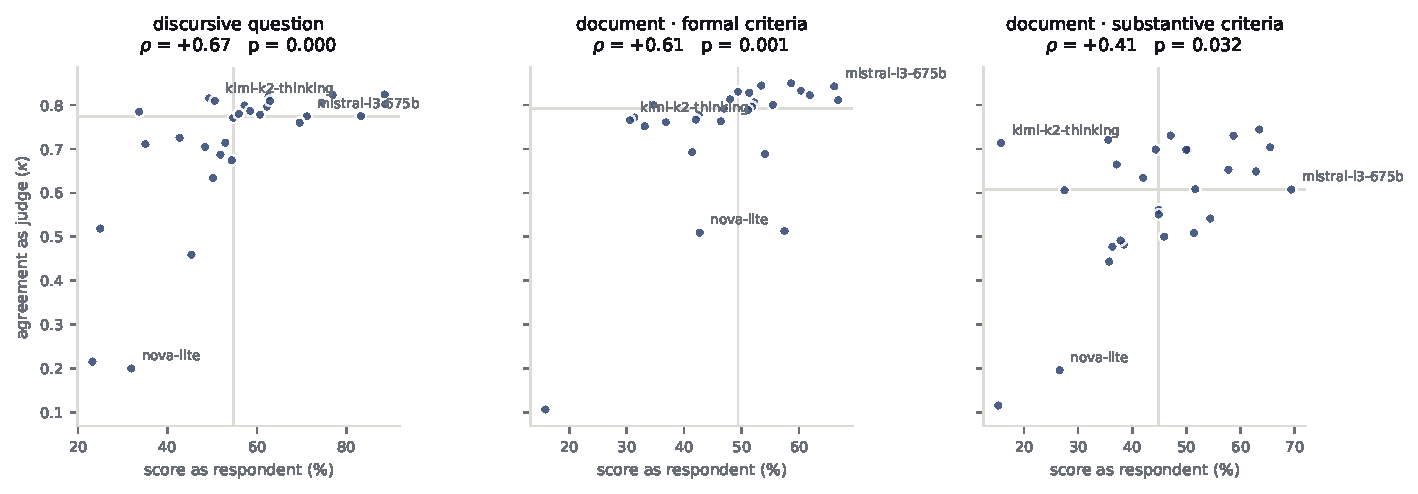
\includegraphics[width=\textwidth]{../artigo2_en/papeis}
\caption{Judging against answering, one panel per task. Each point is a model: score as a respondent on the horizontal axis, agreement as a judge on the vertical. Grey lines are the medians. The association weakens from left to right, as the task stops demanding form and starts demanding substance.}
\end{figure}


Spearman's correlation is \textbf{+0.67} on the discursive question (n = 29, p = 0.0001), \textbf{+0.61} on the formal criteria of the document (n = 27, p = 0.0008) and \textbf{+0.41} on the substantive ones (n = 27, p = 0.032). All three are positive, and the order among them is the result: the more the task demands judgment of a thesis and the less it demands conformity to a form, the less performance on the task predicts competence at judging it. It is the same axis that separates form from substance in Section 4.3, now seen from the other side. The quadrant of good judges that answer badly is populated in all three panels, and the counterexamples are strong. \texttt{kimi-k2-thinking} is among the best judges of documents and is last at writing them, with 15.8\% of the substantive points. \texttt{mistral-l3-675b} is first at writing documents and fourteenth as a judge. Under selection by task performance, the two would have been ranked the other way round. Whether the association on substance is genuinely weaker than on the discursive question is undecidable at our sample size: Steiger's test for dependent correlations [9] falls 0.005 short of the conventional cut, and the confidence interval of the difference by resampling runs from -0.18 to +0.55. What holds is that the association exists, is positive, and is too weak on substance to replace calibration against humans.

\section{Discussion}

The three measurements point the same way by independent routes: the legal competence of a language model is not a single quantity, and the convention of reporting it as one number per model and per task erases exactly the differences that matter to whoever will use the result. Writing the correct document and judging whether someone else's document is correct are competences associated at $\rho$ = 0.41 on the part that decides the score. Getting the addressing right and getting the thesis right are measures that order differently and have different leaders. And the same judge, on the same task, agrees with the human very differently depending on the area of law, with a median range of 0.279 within one of the top nine, against 0.047 of distance among those same nine.

The most direct practical consequence concerns the choice of judge. The question "which is the best judge" is ill-posed before the answer is measured, because aggregate agreement is a weighted mean that reflects above all the most numerous subtask: here, the substance class has 413 of the 561 criteria and determines 98\% of the ordering. The answerable question is which is the best judge for the subtask and the area that matter, and it has different answers. When an external decomposition is available, and the grading guidelines of an examining board are a ready-made decomposition the researcher did not invent, decomposing before choosing costs little and changes the choice.

The second consequence concerns what can be published as an ordering. In the data here, the order at the top is not informative: nine judges are within each other's noise on document substance, and the order among them changes from run to run. What we propose is not to abandon the table, but to accompany it with the noise floor and to mark which positions are distinguishable. It is cheap: it requires repeating the protocol, which careful work already does, and converting the resulting dispersion into a threshold, which almost nobody does. Reproducibility has at least three layers and the field reports one. The first is the seed, the only one reported regularly, and fixing it does not solve the problem. The second is batch size: with a fixed seed and temperature zero, the output still depends on what it was processed alongside. This is not a defect, it is floating-point arithmetic, and it has no trivial fix, but it is reportable. The third is the identity of the model, and it is the most serious, because no discipline of code resolves it: the object measured sits on the other side of an application programming interface, and the same name two months later is another model or another implementation, with no way to know which. A published $\kappa$ value is verifiable within a window of time and an inference configuration that nobody describes in full.

\section{Limitations}

The gold standard has three annotators and was not extended: the 940 annotations are inherited from Rabula [5], and the ceiling of the experiment is the same as the original one, the agreement among the three annotators, at 0.789 and 0.763. The benchmark has 105 questions and seven areas, which is little for the readings by area, where each cell rests on 15 questions; the extension to 314 questions is planned. The noise floor was measured in the best case: the value of 0.0101 measures only the variation under repeated inference with frozen code, and does not include variation from a change of prompt, of library or of model version, so the real floor across laboratories is necessarily higher and was not measured. For the same reason, the two-month drift was observed in one model and not measured systematically. All judges received a single formulation of the judging prompt, and it is possible that some respond better to another and that the order changes with it, which was not tested. Finally, the comparison among the correlations of the three panels of Figure 1 is limited by sample power, as Section 4.4 itself states.

\section{Conclusion}

We measured 31 language models in three roles over the same legal material, the same 105 questions from the second stage of the OAB Bar Exam and the same 940 criteria of the official guidelines, with a gold standard from 3 legal experts, and we report the three roles by area of law and by class of criterion. Knowing how to write a legal document and knowing how to judge someone else's are associated competences, and the association weakens as the task stops demanding form and starts demanding substance, from $\rho$ = 0.67 on the discursive question to 0.41 on the substantive criteria of the document. Document drafting is not a single task for measurement purposes: split into the classes the board labels, it produces two orderings that agree at $\rho$ = 0.48 and have different leaders. And the agreement of a single judge varies across areas of law far more than the top judges vary among themselves, which makes a single number per judge an insufficient description of the ruler.

Three reporting recommendations follow, and none requires new data. Report the agreement table accompanied by the noise floor, marking which positions are distinguishable, because in ours the top nine are not. Decompose the task before choosing the judge whenever an external decomposition is available, because aggregate agreement reflects the most numerous subtask and not necessarily the one that matters. And treat batch size as part of the protocol, alongside temperature and seed, because it also determines the output. All of them require only reporting what has already been measured and is currently discarded.

\section*{Acknowledgements and declarations}

\textbf{Use of generative AI.} Generative models are the object of study of this work, in the three roles described in Section 3.3, and every number reported comes from running the deposited code over the deposited judgments. In addition, the authors used a language model to assist in writing the analysis and manuscript-assembly code, and in drafting and translating the text, composed first in Portuguese. No number was transcribed by hand, and each reference was checked against the primary source. The authors reviewed and edited all content and take full responsibility for it.

\begin{thebibliography}{99}
\bibitem{r1} Zheng, L., Chiang, W.-L., Sheng, Y., Zhuang, S., Wu, Z., Zhuang, Y., Lin, Z., Li, Z., Li, D., Xing, E. P., Zhang, H., Gonzalez, J. E., Stoica, I. \emph{Judging LLM-as-a-Judge with MT-Bench and Chatbot Arena}. NeurIPS, 2023.
\bibitem{r2} Guha, N. et al. \emph{LegalBench: A Collaboratively Built Benchmark for Measuring Legal Reasoning in Large Language Models}. NeurIPS Datasets and Benchmarks, 2023.
\bibitem{r3} Pires, R., Malaquias Junior, R., Nogueira, R. \emph{Automatic Legal Writing Evaluation of LLMs}. ICAIL '25: Proceedings of the Twentieth International Conference on Artificial Intelligence and Law, 420--424, 2025. doi:10.1145/3769126.3769227.
\bibitem{r4} Pires, R., Sales Almeida, T., Larcher Junior, C., Bonás, G., Abonizio, H., Piau, M., Malaquias Junior, R., Laitz, T., Nogueira, R. \emph{Magis-Bench: Evaluating LLMs on Magistrate-Level Legal Tasks}. arXiv:2605.08437, 2026.
\bibitem{r5} Pacheco, E. C. B., Suriani, F. M., Ribeiro, R. \emph{Rabula: A Benchmark for Evaluating LLMs in Brazilian Legal Tasks}. Proceedings of the First Argument Mining and Empirical Legal Research Workshop (AMELR 2025), CEUR-WS Vol-4089, paper 6, 2025.
\bibitem{r6} Goldberg, D. \emph{What Every Computer Scientist Should Know About Floating-Point Arithmetic}. ACM Computing Surveys, 23(1), 5--48, 1991.
\bibitem{r7} Cohen, J. \emph{A Coefficient of Agreement for Nominal Scales}. Educational and Psychological Measurement, 20(1), 37--46, 1960.
\bibitem{r8} Fleiss, J. L. \emph{Measuring Nominal Scale Agreement Among Many Raters}. Psychological Bulletin, 76(5), 378--382, 1971.
\bibitem{r9} Steiger, J. H. \emph{Tests for Comparing Elements of a Correlation Matrix}. Psychological Bulletin, 87(2), 245--251, 1980.
\bibitem{r10} Pacheco, E., Russo, C. M. \emph{Synthetic corpora in the adaptation of language models to Brazilian law}. Companion article, in preparation, 2026.
\bibitem{r11} Pacheco, E., Russo, C. M. \emph{Agreement of 31 candidate automatic judges against a human gold standard on Brazilian legal tasks}, v1.0 [Data set]. Zenodo, 2026. doi:10.5281/zenodo.22739161.
\bibitem{r12} Pacheco, E., Russo, C. M. \emph{Paired raw and structured corpora for Brazilian legal domain adaptation}, v1.0 [Data set]. Zenodo, 2026. doi:10.5281/zenodo.22739216.
\bibitem{r13} Pacheco, E., Russo, C. M. \emph{Judgments of 180 trained conditions on a Brazilian Bar Examination benchmark}, v1.0 [Data set]. Zenodo, 2026. doi:10.5281/zenodo.22739184.
\bibitem{r14} Pacheco, E. \emph{Measuring the competence of LLMs in Brazilian law} [Source code]. github.com/eduardocbpacheco/measuring-llm-competence-brazilian-law, 2026.
\end{thebibliography}
\end{document}
